\chapter{Training Data Creation}
\label{ch:dataset-creation}

In this Chapter, we describe how we created our training dataset and the gold standard that we use in the upcoming Chapters
to train and evaluate different taxonomy matching approaches.
First, we will look at different approaches on how to use the Semantic Web to generate an extensive collection
of product data and use annotated identifiers to match products across different e-commerce platforms.
Next, we describe how those instance pairs were used to create a training dataset of two classes that are part
of different e-commerce taxonomies and a corresponding label that indicates if those classes are equal to each other,
if one class contains the other or if they are disjoint.
Furthermore, we introduce a method to provide edge case examples that are close to our positive labels (\emph{equal}, \emph{contains},
\emph{contained-in}), but are actually \emph{disjoint}.
This Chapter is concluded by an overview of the inherent statistics of our gold standard.
Here, we describe the depth of the covered taxonomies and visualize the distribution of labels.

\section{Retrieving Product Information from the Semantic Web}
\label{sec:retrieve-product-semantic-web}

This Section outlines an approach to retrieve product specific information from the Semantic Web.
The first approach is based on the work of the WDC project and a second approach crawls large
retailers directly and extracts the data we are interested in.

\subsection{Web Data Commons Product Dataset and Gold Standard}

As outlined in Section~\ref{sec:semantic-web} the Semantic Web provides machine-readable information in annotated
HTML-code.
The WDC project provides class-specific datasets that are based on schema.org data and extracted from the
Common Crawl corpus~\cite{meusel2014webdatacommons}.
In addition, Petrovski et al.\@~\cite{petrovski2016wdc} created a gold standard that contains product matches
based on shared identifiers and other indicators.

For this Thesis, the product class-specific dataset is used, which contains about 300 million products stored as
quads.
The file layout is "$<$subject$>$ $<$predicate$>$ $<$object$>$ $<$source$>$ .", e.g.,
"\_:nodeabcd $<$http://schema.org/Product/name$>$ 'Soccer Ball' $<$http://123stores.com/shopby/?brand=1214$>$ .".

There are multiple ways to describe the class of a product in the schema.org notation.
The most used properties are "Category", "Breadcrumb", and the use of a "BreadCrumbList" that links to the individual
levels of the class hierarchy.
As a first step, the quads were parsed and a set of $<$nodeId$>$, $<$breadcrumb$>$ tuples created that were joined
with the WDC gold standard for product matching~\cite{petrovski2016wdc}.
This resulted in a dataset that contains the productId, the source URI, and the class of the product.
Using the clusters of the WDC gold standard it was also possible to assign a high-level category to each product.
Next, a self-join with the dataset is performed to create product pairs that can later be labelled.

Unfortunately, the resulting dataset is to small for the remaining analysis.
Most PLDs contain only a few products.
Hence, we favor the approach introduced in the next Section in which we prefer a deep crawl of individual pages
over a broad crawl across the web.

\subsection{Crawling Product Data from the Semantic Web}

Another way to get product data from the web is a self-written crawler that targets e-commerce sites directly.
The Common Crawl corpus has a broad coverage of different domains, but the number of pages per domain is
comparatively small.
A self-written crawler has the advantage that all sub-pages of a domain can be crawled and only the content of
interest is extracted.

Scrapy is an "open source [\ldots] framework for extracting the data you need from websites.
In a fast, simple, yet extensible way"~\cite{scrapy}.
The data of the following PLDs was crawled as a foundation for our experiments:
amazon.com, walmart.com, ebay.com, bestbuy.com, newegg.com, and overstock.com.

Since the number of PLDs that were crawled is small, there was no need for a generic schema.org extraction framework
like LDSpider~\cite{isele2010ldspider}.
Instead, we use XPath to parse the Document Object Model (DOM)-tree of an HTML-file to get
the relevant properties per page.
Those were the identifiers, the class, and the source-URI of the product.
Again, a self-join over the identifiers resulted in product pairs.

This Section introduced two approaches to generate a set of product-pairs that have the same underlying
entity, identified by a set of product identifiers, and distinct categories that were assigned by the individual
online-shops.

\section{Assigning Semantic Labels to Class-Pairs}

In this Section, a method is introduced to transform the product-pairs into class-pairs with a semantic label.
A sample from the resulting training dataset is provided in Table~\ref{tab:goldstandard-example}.
\begin{table}[htbp]
    \begin{tabularx}{\textwidth}{lXlX|l}
        pld\_l & class\_l & pld\_r & class\_r & label \\
        \hline
        amazon & [\ldots] Women $>$ Smartwatches & bestbuy & [\ldots] All Smartwatches & contained-in \\
        amazon & [\ldots] Binocular, Camera \& Camcorder Straps & bestbuy & [\ldots] Camera Straps & equal \\
    \end{tabularx}
    \caption{Training Dataset Sample.}
    \label{tab:goldstandard-example}
\end{table}
Table~\ref{tab:goldstandard-example} consists of five columns.
"pld\_l" and "pld\_r" indicate the source of the left and right class labels.
"class\_l" and "class\_r" are the hierarchical class-labels, where $>$ indicates the different categories.
For the visualisation, we removed the first parts of the class-labels.
Finally, "label" is the label that our approach assigned.
The remainder of this Section will cover the creation of this training dataset based on the product-pairs.

Following Euzenat and Shvaiko~\cite[p. 113]{euzenat2007ontology} "[the] easiest way to compare classes when they share instances
is to test the intersection of their instance set A and B and to consider that these classes are very
similar when $A \cap B = A = B$, more general when $A \cap B = B$ or $A \cap B = A$."
It is, therefore, possible to infer the label with the set relation.
$A \cap B = A = B$ indicates equality, $A \cap B = B$ and $A \cap B = A$ indicate that A contains B and
A is contained in B, respectively, and, finally, $A \cap B =  \emptyset$ indicates disjointness.
The term \emph{overlap} is used in case none of the above conditions hold~\cite{larson1989theory}.
An overlap occurs when the classes have some products in common, but both classes contain products that also
have other classes in the other taxonomy.

As the next step, the labels for each class-label pair were computed.
Algorithm~\ref{alg:goldstandard-creation} provides pseudo-code for the labelling of the training dataset.
\begin{algorithm}{\MYCALL{Training Dataset}{$tuples$, $pld\_pairs$}}
\caption{Class-Label Pair Labelling}
\label{alg:goldstandard-creation}
\begin{algorithmic}[1]
\LOOP
	\FOR{$pair \leftarrow pld\_pairs$}
		\FOR{$class\_l \leftarrow tuples.pld[pair[0]]$}
			\FOR{$class\_r \leftarrow tuples.pld[pair[1]]$}
				\STATE $left \leftarrow tuples.class[class\_l]$
				\STATE $right \leftarrow tuples.class[class\_r]$
				\STATE $intersection \leftarrow tuples.class[class\_l \& class\_r]$

				\IF{$intersection = \emptyset$}
					\RETURN $disjoint$
				\ENDIF
				\IF{$intersection = left = right$}
					\RETURN $equal$
				\ENDIF
				\IF{$intersection = left$}
					\RETURN $contained-in$
				\ENDIF
				\IF{$intersection = right$}
					\RETURN $contains$
				\ENDIF
				\RETURN $overlap$
			\ENDFOR
		\ENDFOR
	\ENDFOR
\ENDLOOP
\end{algorithmic}
\end{algorithm}

For every PLD-pair, every possible class-label pair is computed.
Then, for each class-label pair, the set of product-pairs with a match of the left
class and the set of product-pairs with a match of the right class is computed.
Those are called left and right in the algorithm.
Finally, the set of product-pairs with a match of the left and the right class
are computed and the set logic from above is applied to assign the labels.

Using this setup, each possible class-pair per PLD-pair gets a label that depends on
the number of shared instances.

In this Section a setup was introduced to transform the product-pairs from Section~\ref{sec:retrieve-product-semantic-web}
into a labelled training dataset that consists of class-pairs with a label indicating that two
classes are equal or disjoint or if one class is more general than the other.

\section{Generating Corner-Cases}
\label{sec:corner-cases}

During the creation of the training dataset, we pair all different class labels between two taxonomies and assign a label
to each of those pairs stating if they are equal or if one contains the other or if they are disjoint.
We plan to use this labelled data for the training and evaluation of taxonomy matching methods.

This results in a huge amount of negative data samples since it will also include obvious mismatches like
"Clothing $>$ Pants $>$ Mens Jeans" and "Electronics $>$ Camera \& Photo $>$ Digital Cameras".
Hence, it is likely that the algorithm will have an easy time to label those as \emph{disjoint} examples and may not be
able to identify the most discriminating features to classify positive classes.

A common approach to tackle this problem is the inclusion of edge-cases in the training data.
Those are samples that are very close to the positively labelled instance, but should receive a negative prediction
from the matcher.
Therefore, we generate artificial edge-cases for the \emph{disjoint} label and add those to our training data.
Since we are interested in samples that are close, but \emph{disjoint}, we use the taxonomic structure of the instances
that are already part of our training dataset.
The tree structure below illustrates a fictitious taxonomy from an electronic e-commerce platform.
\begin{verbatim}
Electronics
|- Cameras
|   |- Digital Cameras
|   |- Polaroid Cameras
|- TVs
\end{verbatim}
Instead of searching across two taxonomies for edge-cases, we simply add leaves in the taxonomy tree that share a parent
and label them as \emph{disjoint}.
In the example above, the class-labels for "Electronics $>$ Cameras $>$ Digital Cameras" and for
"Electronics $>$ Cameras $>$ Polaroid Cameras" are close, but we can be certain that they are \emph{disjoint}.

We search through the complete training dataset that we derived from the Semantic Web for class-label pairs that share
their immediate parent and add those as additional edge-cases to the training dataset.

\section{Class Label Balancing}
\label{sec:label-balancing}

Including the edge-cases, as described in Section~\ref{sec:corner-cases}, the training set consists of
1,057 positive examples and 1,030,497 negative examples.
Out of those 1,030,497 negative examples, 25,674 were artificially generated.
This results in a ratio of 1 positive example for 947 negative examples.

Many machine learning algorithms struggle if the number of class-labels are significantly
imbalanced~\cite{chawla2002smote}.
On the one hand, the training time increases significantly, since more examples have to be processed,
but most of the negative examples may have a low information content, as the disjoint example given at the beginning of the
previous Section illustrates.
On the other hand, there may not be enough positive examples to learn relevant features for the classification.
We will introduce the two approaches we use to mitigate those problems in this Section.

First, we use under-sampling approaches to reduce the number of negative samples~\cite{chawla2002smote}.
Out of all actual \emph{disjoint} pairs (excluding artificially generated edge-cases), we retain 0.5 percent.
From the generated \emph{disjoint} pairs, we retain 10 percent.
We provide a fixed random-seed for the sampling to make sure that the experiment results are deterministic across
multiple runs and are not influenced by different samples.
Overall, this reduces the number of \emph{disjoint} pairs in our training set to 5784
and results in a ratio of 1 positive example for about 6 negative examples.

We use the resulting, smaller dataset for the training and evaluation of all text-based taxonomy matching models.
Since the training data is used to find an optimal decision threshold, the value added by additional positive samples
(over-sampling) is negligible.

The machine learning algorithms also profit from additional positive examples.
In  addition to the under-sampling of the majority class, we add over-sampling of the minority classes.
Chawla et al.\@~\cite{chawla2002smote} introduce the Synthetic Minority Over-sampling TEchnique (SMOTE) and show
that the "combination of SMOTE and under-sampling performs better than plain under-sampling".
They also prove that synthetic minority examples generated by SMOTE improve the classification performance of multiple
machine learning models compared to over-sampling by replicating positive instances.

To generate new samples, SMOTE takes multiple instances of the minority class in a nearest-neighbors fashion and interpolates
a new example at a random point between these two.
This creates artificial positive examples to balance the class-distribution during the training of machine learning models.

In this Section, we introduced two approaches for dealing with our imbalanced training data.
We used random under-sampling during the training of text-based classifiers and, in addition, over-sampling with
SMOTE for the machine learning models.
We expect that under-sampling of \emph{disjoint} class-label pairs reduces the overall training time without sacrificing
performance.
The over-sampling based on SMOTE should increase the performance of the machine learning models since they will have
more positive training data.

\section{Gold Standard Creation and Dataset Statistics}
\label{sec:goldstandard-statistics}

In addition to the automatically labelled product class-label pairs, we manually checked 739 positive product class-label
pairs and updated their label if necessary.
Since two classes are only labelled as \emph{disjoint} by Algorithm~\ref{alg:goldstandard-creation} if they have no instances
in common, and we also create artificial corner-cases that are guaranteed to be disjoint, we have high confidence
that \emph{disjoint} labels are assigned correctly.
Yet, we found that the instance-based automatic annotation assigns wrong labels if one e-commerce platform has many
products in a certain class and the other only a few.
In those cases, an \emph{equal} class-label pair may still receive a \emph{contains} or \emph{contained-in} label.
To avoid those pitfalls and get a high-quality dataset for our evaluation, we created a gold standard from the training
dataset.

In the remainder of this Section, we present the properties of the gold standard that we use for the evaluation of
the taxonomy matching algorithm that we describe in the upcoming Chapter.
Overall it contains 241 \emph{equal}, 257 \emph{contains}, 241 \emph{contained-in}, and 5045~\emph{disjoint} class-label
pairs.

Figure~\ref{fig:label-distribution} illustrates the distribution of the positive labels between different PLD-pairs.
We can see that the PLD-pairs "(amazon, ebay)" and "(bestbuy, ebay)" have comparatively few \emph{contains} class-label
pairs.
This indicates that amazon and bestbuy use higher-level classes, compared to fine-granular class-labels for ebay.
Apart from those two PLD-pairs, every positive label has at least ten instances for each PLD-pair.
\begin{figure}[!htbp]
	\centering
	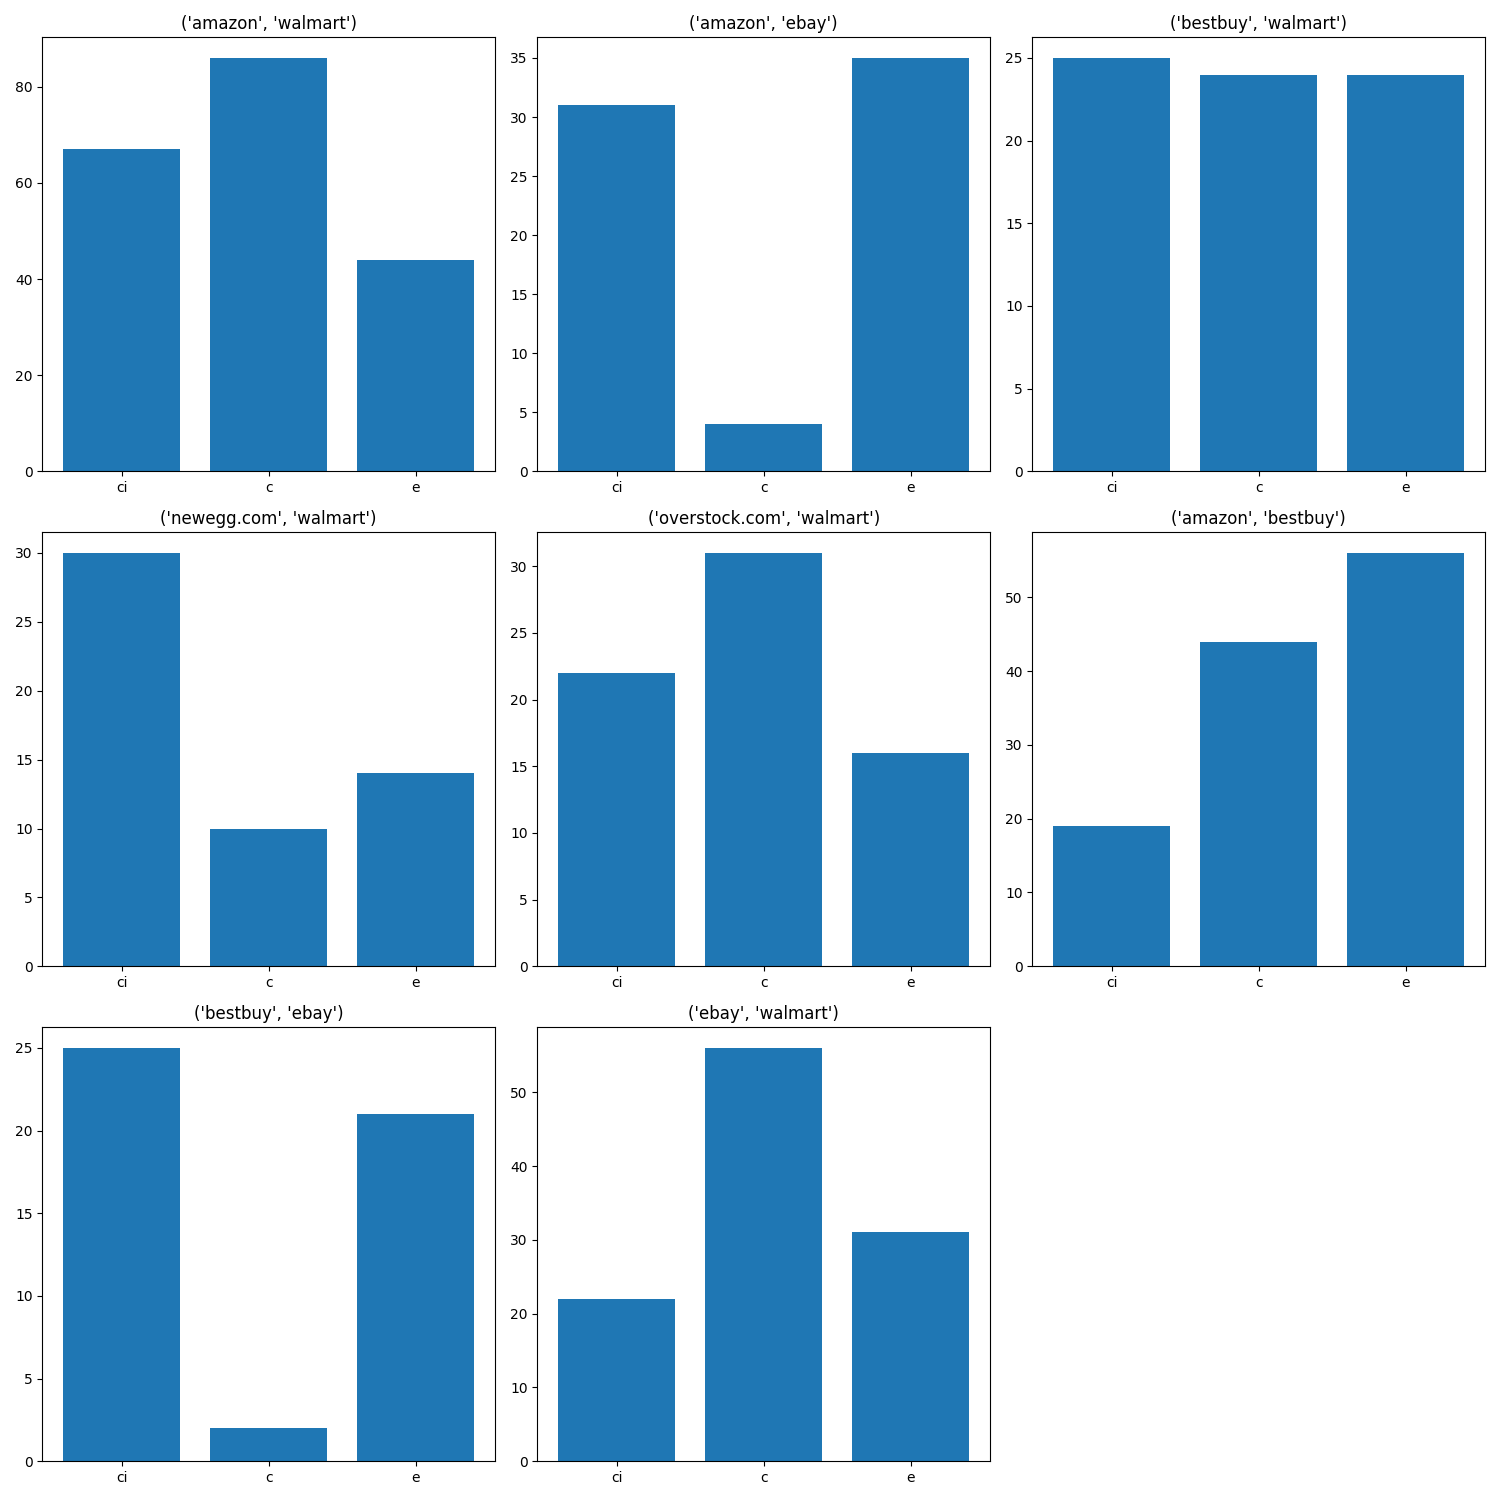
\includegraphics[width=13cm]{images/label-distribution.png}
	\caption{Label Distribution across PLD-Pairs.}
	\label{fig:label-distribution}
\end{figure}

We use those PLD-pairs for nested cross-validation during our experiments.
To use all gold standard examples during the training and the evaluation, we hold out one of the seven PLD-pairs
for each training session and use it to evaluate the models afterwards.
We aggregate those intermediate results to arrive at the numbers we present in Chapter~\ref{ch:experiment-results}.
In each iteration, we use the remaining six PLD-pairs to train our models and perform $k$-fold cross-validation
to optimize hyperparameters.

While the GPC standard uses only three hierarchy-levels for their product class-labels, our dataset indicates that
real-world e-commerce platforms use deeper taxonomies.
Figure~\ref{fig:depth-distribution} visualizes the number of categories per class-label.
We see that a class-label consists of 4 to 5 categories on average.
\begin{figure}[!htbp]
	\centering
	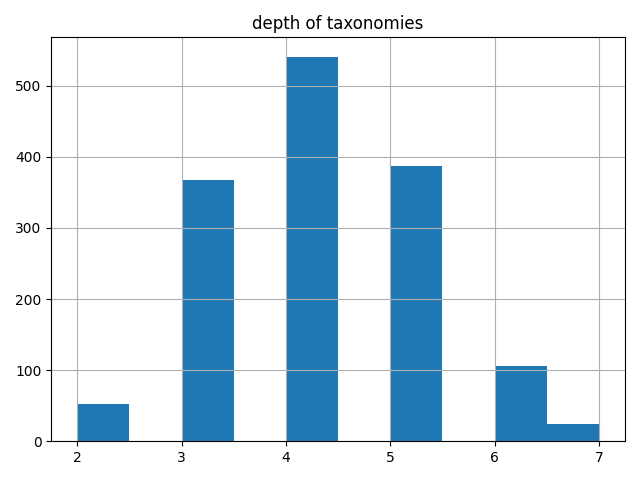
\includegraphics[width=8cm]{images/depth-distribution.png}
	\caption{Depth Distribution of Class-Labels.}
	\label{fig:depth-distribution}
\end{figure}
This indicates that previous contributions in the taxonomy matching domain that use the GPC may make the simplifying
assumption that a class-label consists of at most three categories.
Therefore, their results may not hold up on real-world taxonomies from large e-commerce platforms.

% amazon	Sports & Outdoors > Sports & Fitness > Exercise & Fitness > Clothing > Men > Pants	1	walmart	Clothing > Fashion Brands > Under Armour > Men's	5	1	contained-in    contained-in
% amazon	Beauty & Personal Care > Tools & Accessories > Makeup Brushes & Tools > Eye > False Eyelashes & Adhesives	1	walmart	Clothing > Mens Clothing > Mens Socks > Mens Socks	5	1	contained-in
% bestbuy	TV & Home Theater > TVs > 4K Ultra HD TVs	1	walmart	Electronics > TV & Video > Shop TVs by Size > 55 Inch TVs	1	1	equal
% bestbuy	TV & Home Theater > Projectors & Screens > Projector Mounts	1	walmart	Electronics > Home Audio & Theater > Home Theater > Projectors > Projectors	3	1	contained-in
% bestbuy	Cameras & Camcorders > Digital Cameras > Mirrorless Cameras	3	walmart	Electronics > Cameras & Camcorders > Mirrorless Cameras	1	1	contains    equal
% bestbuy	Cameras & Camcorders > Digital Cameras > Mirrorless Cameras	3	walmart	Electronics > Cameras & Camcorders > Digital SLR Cameras	1	1	contains    contains
